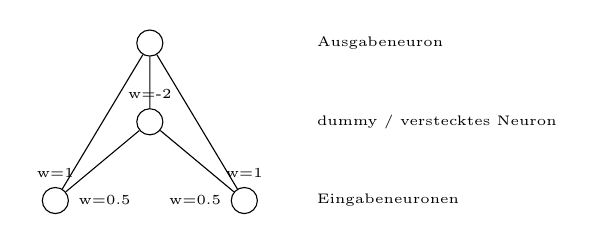
\begin{tikzpicture}[font=\tiny]
	\node (out) at (0,0) [draw,circle]{};
	\node (hidden) at (0,-1) [draw,circle,
		label=above:{w=-2}]{};
	\node (in1) at (-1.2,-2) [draw,circle,
		label=above:{w=1}]{};
	\node (in2) at (1.2,-2) [draw,circle,
		label=above:{w=1}]{};

	\draw (in1.east) node[ right] {w=0.5};
	\draw (in2.west) node[ left] {w=0.5};

	\draw (out) +(2,0) node[right] {Ausgabeneuron};
	\draw (hidden) +(2,0) node[right] {dummy / verstecktes Neuron};
	\draw (hidden) +(2,-1) node[right] {Eingabeneuronen};

	\draw (in1) -- (hidden) -- (out);
	\draw (in1) -- (out);
	\draw (in2) -- (hidden);
	\draw (in2) -- (out);
\end{tikzpicture}
